\documentclass[12pt,fleqn]{article}\usepackage{../common}
\begin{document}
Bir Coklu Ikisel Dagilim (Multivar. Binary Distribution) ve Boltzmann Dagilimi

$$  
\mlabel{3}
P(x;W) = \frac{1}{Z(W)} 
\exp \bigg[ \frac{1}{2} x^T W x \bigg]
$$

ki $W$ simetrik ve caprazinda (diagonal) sifir iceren bir matristir. 

Olurluk (likelihood)

$$  
\prod _{n=1}^{N} P(x^{(n)};W) = \frac{1}{Z(W)} 
\exp \bigg[ \frac{1}{2} x^{(n)^T} W x^{(n)} \bigg]
$$

Log olurluk

$$  
\mlabel{1}
\mathcal{L} = \ln \big( \prod _{n=1}^{N} P(x^{(n)};W) \big) = 
\sum _{n=1}^{N} \bigg[ \frac{1}{2} x^{(n)^T} W x^{(n)} - \ln Z(W) \bigg]
$$

Birazdan $\frac{\partial \mathcal L}{\partial w_{ij}}$ turevini alacagiz, o sirada $\ln Z(W)$'nin turevi lazim, 
daha dogrusu $Z(W)$'yi nasil turevi alinir hale getiririz?

$Z(W)$ normalizasyon sabiti olduguna gore, dagilimin geri kalaninin
sonsuzlar uzerinden entegrali (ya da toplami) normalizasyon sabitine
esittir, 

$$ 
Z(W) = \sum_x  \exp \bigg[ \frac{1}{2} x^T W x \bigg]
 $$

$$ 
\ln Z(W) = \ln \bigg[ \sum_x  \exp \big( \frac{1}{2} x^T W x \big) \bigg]
 $$

Log bazli turev alinca log icindeki hersey oldugu gibi bolume gider, ve log
icindekinin turevi alinirak bolume koyulur. Fakat log icine dikkatli
bakarsak bu zaten $Z(W)$'nin tanimidir, boylece denklemi temizleme sansi
dogdu, bolume hemen $Z(W)$ deriz, ve turevi log'un icine uygulariz,


$$ 
\frac{\partial}{\partial w_{ij}} \ln Z(W) = 
\frac{1}{Z(W)}
\bigg[ 
\sum_x \frac{\partial}{\partial w_{ij}} \exp \big( \frac{1}{2} x^T W x \big) 
\bigg]
 $$


$$ 
\mlabel{2}
\frac{\partial}{\partial w_{ij}} \exp \big( \frac{1}{2} x^T W x \big)  = 
\frac{1}{2}  \exp \big( \frac{1}{2} x^T W x \big) 
\frac{\partial}{\partial w_{ij}}x^T W x
$$

(2)'in icindeki bolumu acalim,

$$ \frac{\partial}{\partial w_{ij}}x^T W x = x_i x_j $$

Simdi (2)'ye geri koyalim,

$$ =  \frac{1}{2}  \exp \big( \frac{1}{2} x^T W x \big) x_i x_j$$

$$ 
\frac{\partial}{\partial w_{ij}} \ln Z(W) = 
\frac{1}{Z(W)}
\bigg[ 
\sum_x \frac{1}{2}  \exp \big( \frac{1}{2} x^T W x \big) x_i x_j
\bigg]
$$

$$ 
= 
\frac{1}{2}  \sum_x \frac{1}{Z(W)}  \exp \big( \frac{1}{2} x^T W x \big) x_i x_j
$$

$$ 
= 
\frac{1}{2}  \sum_x P(x;W) x_i x_j
$$

Ustteki son ifadede bir kisaltma kullanalim,

$$ 
\sum_x P(x;W) x_i x_j =  <x_i,x_j>_{P(x;W)}
$$

Artik $\ln Z(W)$'nin turevini biliyoruz. O zaman tum log olurlugun turevine
(1) donebiliriz, 

$$  
\frac{\partial \mathcal{L}}{\partial w_{ij}} = 
\sum _{n=1}^{N} \bigg[ 
\frac{\partial}{\partial w_{ij}}  \frac{1}{2} x^{(n)^T} W x^{(n)} - 
\frac{\partial}{\partial w_{ij}}  \ln Z(W) \bigg]
$$


$$  
=
\sum _{n=1}^{N} 
\bigg[ 
\frac{1}{2} x_i^{(n)^T}x_j^{(n)} - 
\frac{\partial}{\partial w_{ij}}  \ln Z(W) 
\bigg]
$$

$$  
=
\sum _{n=1}^{N} 
\bigg[ 
\frac{1}{2} x_i^{(n)^T}x_j^{(n)} - 
\frac{1}{2}<x_ix_j>_{P(x;W)}
\bigg]
$$ 

1/2 sabitlerini atalim, 

$$  
=
\sum _{n=1}^{N} 
\bigg[ 
 x_i^{(n)^T}x_j^{(n)} - <x_ix_j>_{P(x;W)}
\bigg]
$$

Eger 

$$
<x_ix_j>_{Data} = \frac{1}{N} \sum _{n=1}^{N}  x_i^{(n)^T}x_j^{(n)}
$$

olarak alirsak, esitligin sag tarafi verisel kovaryansi (empirical
covariance) temsil eder. Duzenleyince,

$$ 
N \cdot <x_ix_j>_{Data} = \sum _{n=1}^{N}  x_i^{(n)^T}x_j^{(n)}
$$

simdi esitligin sag tarafi uc ustteki formule geri koyulabilir,

$$ 
\frac{\partial \mathcal{L}}{\partial w_{ij}}  = 
N \big[<x_ix_j>_{Data}  - <x_ix_j>_{P(x;W)} \big] 
$$

Bu bir gradyan guncelleme formulu olarak gorulebilir, ve $N$ yerine bir
guncelleme sabiti alinabilir. 

Ana dagilim fonksiyonu baz alinarak, yeni veri $x$ uzerinde o $x$ uzerinde
biri haric tum ogelerin bilindigi durumda bilinmeyen tek hucre $i$ icin 1
olma olasilik degeri,

$$ P(x_i = 1 | x_j, j \ne i) = \frac{1}{1 + e^{-a_i}} $$

ve,

$$ a_i = \sum_j  w_{ij}x_j $$

Bu kosulsal olasiligin ne kadar temiz oldugu onemli, ustteki gorulen bir
sigmoid fonksiyonu. Bu fonksiyonlar hakkinda daha fazla bilgi {\em Lojistik
  Regresyon} yazisinda bulunabilir. Ana formul (3)'ten bu noktaya nasil
eristik?

$x$ vektoru icinde sadece $x_i$ ogesinin $b$ olmasini $x^b$ olarak
alalim. Once kosulsal dagilimda ``verili'' olan kismi elde etmek lazim. O
zaman

$$ P(x_j,j \ne i) = P(x^0) + P(x^1) $$

Bu bir marjinalizasyon ifadesi, tum olasi $i$ degerleri uzerinde bir toplam
alinca geri kalan $j$ degerlerinin dagilimini elde etmis oluruz. 

$$  P(x_i = 1 | x_j,j \ne i)  = \frac{P(x^1)}{P(x^0) + P(x^1)} $$

cunku $P(A|B) = P(A,B) / P(B)$ bilindigi gibi, ve $P(x^1)$ icinde $x_1=1$
setini iceren tum veriler uzerinden. 

Esitligin sag tarafinda $P(x^1)$'i bolen olarak gormek daha iyi, ayrica
ulasmak istedigimiz $1/1 + e^{-a_i}$ ifadesinde $+1$'den kurtulmak iyi
olur, boylece sadece $e^{-a_i}$ olan esitligi ispatlariz. Bunun her iki
denklemde ters cevirip 1 cikartabiliriz,

$$  1 / P(x_i = 1 | x_j,j \ne i) = \frac{P(x^0) + P(x^1)}{P(x^1)} 
$$

$$= 
1 + \frac{ P(x^0)}{P(x^1)}
$$

Bir cikartirsak, $\frac{ P(x^0)}{P(x^1)}$ kalir. Bu bize ulasmak
istedigimiz denklemde $e^{-a_i}$ ibaresini birakir. Artik sadece $\frac{
  P(x^0)}{P(x^1)}$'in $e^{-a_i}$'e esit oldugunu gostermek 
yeterli. 


$$ 
\frac{ P(x^0)}{P(x^1)} = \exp( x^{0^T}Wx^0 -   x^{1^T}Wx^1 )
$$

Simdi $x^TWx$ gibi bir ifadeyi indisler bazinda acmak icin sunlari yapalim, 


$$ x^TWx = \sum_{k,j} x_kx_jw_{kj} $$

Ustteki cok iyi bilinen bir acilim. Eger

$$  \sum_{k,j} \underbrace{x_kx_jw_{ij}}_{Y_{kj}} = \sum_{k,j}Y_{kj} $$

alirsak birazdan yapacagimiz islemler daha iyi gorulebilir. Mesela $k=i$
olan durumu dis toplamdan disari cekebiliriz

$$ 
= \sum_{k \ne i}\sum_j Y_{kj} + \sum_{j} Y_{ij}
$$

Daha sonra $j = i$ olan durumu ic toplamdan disari cekebiliriz, 


$$ 
= \sum_{k \ne i}( \sum_{j \ne i} Y_{kj} + Y_{ki}) + \sum_{j} Y_{ij}
$$

Ic dis toplamlari birlestirelim,


$$ 
= \sum_{k \ne i,j \ne i} Y_{kj} + \sum_{k \ne i}  Y_{ki} + \sum_{j} Y_{ij}
$$

$$ 
= \sum_{k \ne i,j \ne i} Y_{kj} + \sum_{k}  Y_{ki} + \sum_{j} Y_{ij} + Y_{ii}
$$

Ustteki ifadeyi $ \exp( x^{0^T}Wx^0 -   x^{1^T}Wx^1 )$ icin kullanirsak,

$$ 
\exp 
\big( 
\sum_{k}  Y_{ki}^0 + \sum_{j} Y_{ij}^0 + Y_{ii}^0 - 
( \sum_{k}  Y_{ki}^1 + \sum_{j} Y_{ij}^1 + Y_{ii}^1  )
\big)
 $$

$\sum_{k \ne i,j \ne i} Y_{kj}$ teriminin nereye gittigi merak edilirse,
bu ifade $i$'ye dayanmadigi icin bir eksi bir arti olarak iki defa dahil
edilip iptal olacakti. 

$$ 
= \exp \big( 
0 - ( \sum_{k}  Y_{ki}^1 + \sum_{j} Y_{ij}^1 + Y_{ii}^1  ) 
\big)
 $$

$W$'nin simetrik matris oldugunu dusunursek, $\sum_{k}  Y_{ki}^1$ ile $\sum_{j}Y_{ij}^1$ ayni ifadedir, 

$$ 
= \exp \big( 
- ( 2 \sum_{j} Y_{ij}^1 + Y_{ii}^1  ) 
\big)
 $$

$W$ sifir caprazli bir matristir, o zaman $Y_{ii}^1=0$, 

$$ 
= \exp \big( 2 \sum_{j} Y_{ij}^1 \big) = \exp (- 2 a_i )
 $$
Orijinal dagilim denkleminde $1/2$ ifadesi vardi, onu basta islemlere dahil
etmemistik, edilseydi sonuc  $\exp (- a_i)$ olacakti. 


\inputminted[fontsize=\footnotesize]{python}{boltz.py}



\begin{minted}[fontsize=\footnotesize]{python}
Y = np.loadtxt('../../stat/stat_mixbern/binarydigits.txt')
label = np.ravel(np.loadtxt('../../stat/stat_mixbern/bindigitlabels.txt'))
Y5 = Y[label==5]
plt.imshow(Y5[0,:].reshape((8,8),order='C'), cmap=plt.cm.gray)
plt.savefig('boltzmann_01.png')

plt.imshow(Y5[1,:].reshape((8,8),order='C'), cmap=plt.cm.gray)
plt.savefig('boltzmann_02.png')

plt.imshow(Y5[2,:].reshape((8,8),order='C'), cmap=plt.cm.gray)
plt.savefig('boltzmann_03.png')
\end{minted}

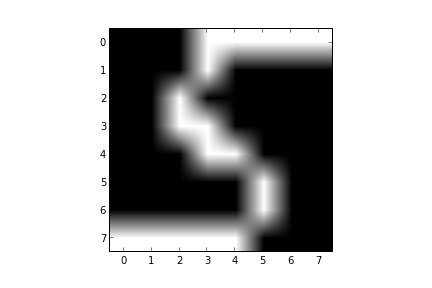
\includegraphics[height=3cm]{boltzmann_01.png}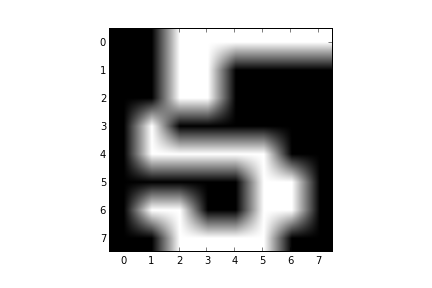
\includegraphics[height=3cm]{boltzmann_02.png}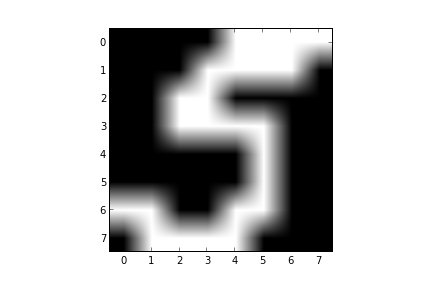
\includegraphics[height=3cm]{boltzmann_03.png}











Information Theory, Inference and Learning Algorithms, D. MacKay

\url{http://nbviewer.ipython.org/gist/aflaxman/7d946762ee99daf739f1}

\url{http://math.stackexchange.com/questions/1095491/from-pxw-frac1zw-exp-bigl-frac12-xt-w-x-bigr-to-sigmoid/}


\end{document}
